\documentclass[11pt]{article}
\usepackage{geometry}                % See geometry.pdf to learn the layout options. There are lots.
\geometry{a4paper}                   % ... or a4paper or a5paper or ... 
%\geometry{landscape}                % Activate for for rotated page geometry
%\usepackage[parfill]{parskip}    % Activate to begin paragraphs with an empty line rather than an indent
\usepackage{graphicx}
\usepackage{amssymb}
\usepackage{epstopdf}
\usepackage[german, english]{babel}
\usepackage[utf8]{inputenc}
\usepackage{hyperref}
\DeclareGraphicsRule{.tif}{png}{.png}{`convert #1 `dirname #1`/`basename #1 .tif`.png}

\title{RoboDucks @ HTL Leonding}
\author{Status Report 2016}
%\date{}                                           % Activate to display a given date or no date

\hyphenation{Le-on-ding}

\begin{document}
\begin{titlepage}
\begin{flushright}

\includegraphics[scale=.85]{../img/htlleondinglogo.png}\\
\end{flushright}

\vspace{3em}

\begin{center}
{\Huge Humanoid Robotics} \\[2em]
\includegraphics[scale=0.55]{img/Titlepage.png}\\[2em]
{\LARGE Status Report 2017}
\end{center}
\end{titlepage}

\section{Introduction}
This report lists the activities of the Humanoid Robotics Team of the year 2017. There is a good number of activities we are proud of to mention here. We also want to be pretty clear that only  a very brief overview is given and many details are left out to keep the report short. If there are any further questions the team lead can be contacted via \\[1em]
Peter Bauer\\
HTL Leonding, Department of Informatics\\
Limesstraße 12 -- 14\\
4060 Leonding\\
Fon: +43 676 6173320\\
Mail: p.bauer@htl-leonding.ac.at

\section{The Name {\em Humanoid Robotics}}
Careful readers may have recognized that the name of our activity has changed from last year's {\em Nao@HTL Leonding} to {\em Humanoid Robotics}. This is due to two facts:
\begin{enumerate}
	\item The HTL Leonding collected all their extra curricula activities under the umbrella of the so-called {\em Program of Excellence}. We are proud to be now a leading part of this program.
	\item The appearance of SoftBank's Nao in our name suggested a single focus on Nao which was considered too much of a restriction, on the one hand. On the other hand, the the name {\em Robotics} would have included industrial robots which are definitely outside of our scope.
\end{enumerate}
Therefore we ended up with {\em Humanoid Robotics} which describes our activities well and gives us enough flexibility for the future.

\section{The Team}
Building a strong team of students and teachers who do a very focused work is one of the key issues we are facing. Especially a smooth hand-over from one student generation to a next is a central topic.
In our current core team
\begin{itemize}
	\item Peter Bauer (Teacher)
	\item Bernhard Bodenstorfer (Teacher)
	\item Sabina Brantner (5AHIF)
	\item Melanie Mühleder (5AHIF)
	\item Viktoria Streibl (5AHIF)
	\item Erik Mayrhofer (3BHIF)
\end{itemize}
we see that three of our students are attending the $5^{\textrm{\small th}}$ grade and will drop out by end of March. Furthermore we have to consider that a high percentage of interested students from last year were not able to continue their engagement in our group due to several reasons. The more we are very happy that one very talented student, Erik Mayrhofer, remained and is now member of the core team.

The more important is it to have again a number of approximately 30 new students who claimed interest in humanoid robotics and joined our team as freshman which makes us still optimistic to keep a sound basis of experienced students and a solid transfer of know how from one generation to the next.

Another new hire we are very happy to have on board is {\em Franz Auernig},  Programming teacher who started to work at the HTL Leonding in fall 2016. He will bring in expertise in the area of embedded programming.

The split of our team into an experienced and a freshman sub team which we introduced last year proved to work well. Therefore we continued this practice. The team of the experienced students are, of course, still working on a software for the Nao Standard Platform League. The freshman team, however, is now to prepare for the Demo Humanoid Challenge which was introduced last year as part of the RoboCup Junior Austrian Open (see section~\ref{sec:demoHumanoidChallenge}).

\section{Co-operations}
With the increasing number of interested students we faced an additional issue this fall, namely to find a common time for our regular meetings. Since it turned out to be impossible to find a common ``hole'' in the schedule of the different students it was necessary to find additional ways to organize regular meetings.

The solution was to organize extra development sprints during the school year scheduled on Fridays, Saturdays or during school holidays where all students are free. To make this offer more attractive we were lucky to partner with {\em Fabasoft} which kindly provides a great working environment and a catering for these extra sprints. The dates for these are/were

\begin{itemize}
	\item December 8 and 9, 2017
	\item January 4 and 5, 2018
	\item February 19 to 23, 2018
	\item March 26 to 29, 2018
\end{itemize}

Our first sprint in December 2017 turned out to be well accepted by the students. We were lucky to count 16 students of the HTL Leonding who spent two days of work although these days were school holidays. Figure~\ref{fig:fabasoft} gives some impression of this event.

\begin{figure}
\begin{center}
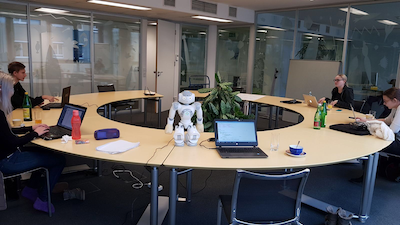
\includegraphics[scale=.574]{img/Fabasoft1.png}
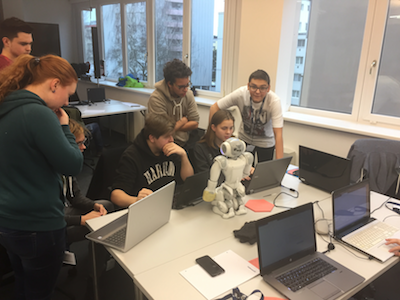
\includegraphics[scale=0.43]{img/Fabasoft2.png}
\end{center}
\caption{Working at Fabasoft}
\label{fig:fabasoft}
\end{figure}

Two further co-operations have been established during this summer with the \foreignlanguage{german}{{\em Pä\-da\-gogische Hochschule der Diözese Linz}} and the {\em Verein RoboCupJunior Austria}. Both contacts came into being under the framework of the RoboCup Junior Austrian Open which will be held in Linz on April 13 and 14, 2018 (see section~\ref{sec:rcj} for further information).

\section{Activities in 2017}
\subsection{Overview}
The following planned activities were done:
\begin{itemize}
	\item {\em Tag der offenen Tür at the HTL Leonding (Jan 26 and 27, 2017):}  As planned we showed our new Naos being able to kick on the newly introduced 8 mm artificial turf. Although the software was not perfect yet it was again a great attraction for all visitors.
		
	\item {\em Messe Jugend und Beruf (October 11 to 14, 2017):}  As every year the Naos were a great attraction to all visitors. The team was able to present a stable software and - as last year - we were happy to face no problems with overheating servos.
	
	\item {\em Increase Marketing Activities:} The focus of activities switched from the promotional video and web site to the organization of the RoboCup Junior Austrian Open (see section~\ref{sec:rcj}). These activities will keep us busy until April 2018. So the original goals were shifted to the year 2018.
\end{itemize}

The planned events {\em RoboCup German Open 2017, Magdeburg (May 5 to 7, 2017)} and  {\em 1. Krone E-Mobility Play Days, Spielberg (September 29 and 30, 2017)} must have been dropped. The main reason was that the effort for designing and programming a soccer software which is in a playable mode was underestimated. Nevertheless we made some significant progress which is described in section~\ref{sec:spl}.

The following extra activities have been accomplished during 2017:

\begin{itemize}
	\item {\em Demo Humandoid Challenge at the RoboCup Junior Austrian Open (April 21 and 22, 2017):} We won the {\bf Second Price} in this newly introduced challenge in the RoboCup Junior (see section~\ref{sec:demoHumanoidChallenge}).
	\item {\em Organization of the RoboCup Junior Austrian Open 2018:} An opportunity to present the HTL Leonding and the Humanoid Robotics initiative to a broader public (see section~\ref{sec:rcj}).
\end{itemize}

\subsection{Demo Humanoid Challenge}\label{sec:demoHumanoidChallenge}
The Demo Humanoid Challenge was introduced during the RoboCup Junior Austrian Open 2017 - held in Weiz. The assignment was to program a shop assistant which can interact with a human customer and present different grocery goods in an arena (see figure~\ref{fig:rcjTraining}). The original challenge was that the placement of the grocery goods on the arena was announced only one hour prior to the competition and the teams had to adapt their software within this timeframe.  We were very proud that our team with Stefan Brandmair and Josef Gruber won the {\bf Second Price} in this challenge.

It is also worth being mentioned that our software was technically the most sophisticated compared to all other teams. This was mainly seen that the adaption of our software took only five minutes, where all other teams had to work hard for two or more hours.

\begin{figure}
\begin{center}
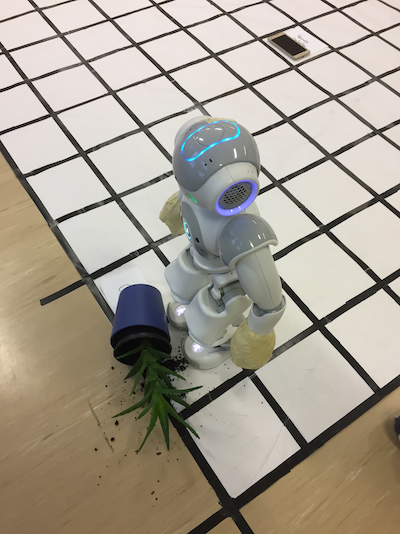
\includegraphics[scale=0.5]{img/RCJTraining.png}
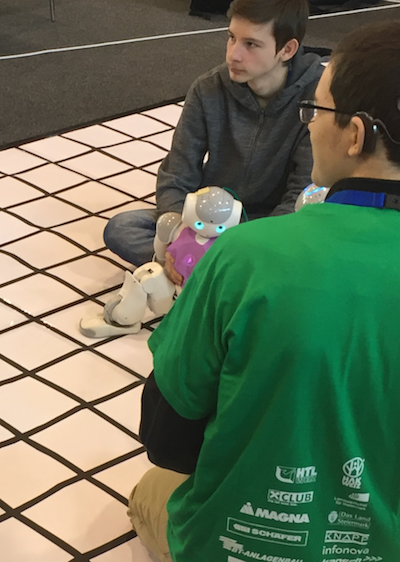
\includegraphics[scale=0.475]{img/RCJ.png}
\end{center}
\caption{Demo Humanoid Challenge 2017}
\label{fig:rcjTraining}
\end{figure}

\subsection{Standard Platform League}\label{sec:spl}
Although we were not able to reach our goals for 2017 the team of Sabina Brantner, Erik Mayrhofer, Melanie Mühleder, and Viktoria Streibl was able to achieve a few important subgoals in our soccer software:

\begin{itemize}
	\item The walk on the 8 mm turf which caused serious troubles during spring and summer this year is now pretty stable. 
	\item The ball recognition and the distance estimation to the ball is also in a very stable state.
	\item The game controller implementation is finished.
\end{itemize}

Currently we are working on the integration of all single software parts and the implementation of a motion controller which will enable us to easier adapt to different grounds and movements.

\subsection{RoboCup Junior Austrian Open}\label{sec:rcj}
During the Austrian Open 2017 in Weiz the idea emerged that the Austrian Open 2018 should be organized in Linz. In co-operation with the Pädagogische Hochschule der Diözese Linz we are busy to make a great event on April 13 and 14, 2018. The Pädagogische Hochschule is the main organizer and supplier of the infrastructure for this. We are supporting in the following areas:

\begin{itemize}
	\item Flexible implementation of time schedules of the different challenges
	\item Resource planning for setup, reduction of arenas, registration desk, etc.
	\item Floor planning and orientation system
	\item Design and manufacturing of the trophies
	\item Communication to the public (Website, promotion, etc.)
	\item Provision of time keepers, referees and other supporting resources
\end{itemize}

\section{Planned Activities for 2018}

\begin{itemize}
	\item {\em Tag der offenen Tür at the HTL Leonding (Jan 25 and 26, 2018):} As usual we will be here and present our latest software. We are currently working hard to integrate our software to show a stable software which makes a Nao kick a goal.
	
	\item {\em RoboCup Junior Austrian Open (April 13 and 14, 2018):}	This event will bind a good number of our resources until end of April. First of all, we plan to send two to three teams to compete in the Demo Humanoid Challenge. Furthermore we continue our efforts to support the organization of this event.
	
	\item {\em Messe Jugend und Beruf (October 10 to 13, 2018):} Another fixed date where we traditionally take part in. Due to a significant change in our team (three students will drop out because they will finish school) we will have some effort to keep the high level of the last years.
	
	\item {\em Marketing Activities:} As mentioned we shifted parts of our activities so we still want to set up a web site and a promotional video in order to make our activities better visible to a wider audience.
\end{itemize}

\section{Acknowledgements}
This project would not be possible without the kind support of several persons and organizations. We would like to express our gratitude to:

\begin{itemize}
	\item \emph{Absolventenverein der HTL Leonding (AbsLeo):} The AbsLeo accompanies this project since 2009. It budgeted the initial hardware which allowed us to get first experience with the Naos and renewed our hardware in Fall 2016. Although it was clear that the whole journey will be a long one we could rely on their constant support. This enabled us to continue our ambitions towards participating the RoboCup World Championships.
	
	\item \emph{Management of the HTL Leonding:} Every project needs the great support from its embedding organization. All the smaller and larger organizational issues we are facing can be solved by means of the friendly support of our school. This is enabled by our head master and the two heads of departments. We are very happy to know that we can rely on them.
	
	\item \emph{Thomas Himmelbauer:} Despite his tough schedule as our school's IT manager he is a great technical supporter of our project. Without him our progress would have never been the one we have. His great expertise in the area of the C++ toolchain as well as his patience to figure out solutions concerning the NaoQi are really priceless.
	
	\item \emph{Fabasoft AG:} The relation to Fabasoft really brought new possibilities to our work. Organizing the extra sprints to make our software better and to bring more students and teams to the field of Humanoid Robotics was a real pleasure. Especially we want to thank Helmut Fallmann for his general support and his goal driven approach, Christian Molnhuber and Sabine Krammer for their operational support. There is no problem that could not be solved with the great help from them.
\end{itemize}

\end{document}  